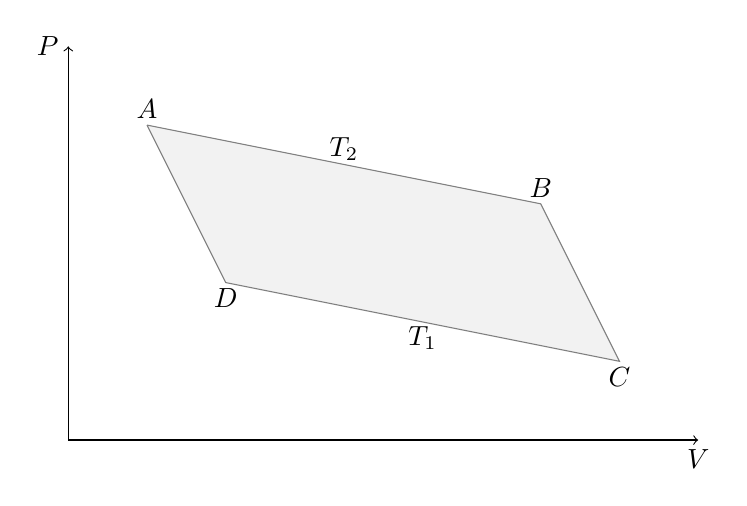
\begin{tikzpicture}[scale=1.0]
  \draw[->] (0,0)--(8,0) node[anchor=north] {$V$};
  \draw[->] (0,0)--(0,5) node[anchor=east] {$P$};
  \draw[gray,fill=gray!10!white] (1,4)--(6,3)--(7,1)--(2,2)--(1,4);
  \draw (1,4.2) node{$A$};
  \draw (6,3.2) node{$B$};
  \draw (7,0.8) node{$C$};
  \draw (2,1.8) node{$D$};
  \draw (3.5,3.7) node{$T_2$};
  \draw (4.5,1.3) node{$T_1$};
\end{tikzpicture}
